
\subsection{Kernels and Trace Kernels}\label{subsec:katk}
As a foundational basis to compute trace alignments, we adapt similarity measures from the database literature.  Given a set of data examples $\mathcal{X}$, (e.g., strings or traces, transition graphs) a (positive definite) \emph{kernel} function $k\colon \mathcal{X}\times \mathcal{X}\to \mathbb{R}$ denotes the similarity of elements in $\mathcal{X}$. If $\mathcal{X}$ is the $d$-dimensional Euclidean Space $\mathbb{R}^d$, the simplest kernel function is the inner product $\Braket{\mathbf{x},\mathbf{x}'}=\sum_{1\leq i\leq d}\mathbf{x}_i\mathbf{x}'_i$.
A kernel is said to \emph{perform ideally} \cite{Gartner03} when $k(x,x')=1$ whenever $x$ and $x'$ are the same object (\textit{strong equality}) and $k(x,x')=0$ whenever $x$ and $x'$ are distinct objects (\textit{strong dissimilarity}). %A kernel is also said to be \emph{appropriate} when similar elements $x,x'\in\mathcal{X}$ are also close in the feature space. Notice that appropriateness can be only assessed  empirically \cite{Gartner03}.
%A positive definite kernel induces a distance metric as:
%
%When the kernel of choice is the inner product, the resulting distance is the Euclidean distance $\norm{\mathbf{x}-\mathbf{x}'}{2}$. A normalized vector $\hat{\mathbf{x}}$ is defined as $\mathbf{x}/\norm{\mathbf{x}}{2}$. For a normalized vector we can easily prove that: $\norm{\hat{\mathbf{x}}-\hat{\mathbf{x}}'}{2}^2=2(1-\Braket{\hat{\mathbf{x}},\hat{\mathbf{x}}'})$.

When $\mathcal{X}$ does not represent directly a $d$-dimensional Euclidean space, we can use an \emph{embedding} $\embed\colon\mathcal{X}\to \mathbb{R}^d$ to define a kernel $k_\embed\colon \mathcal{X}\times \mathcal{X}\to\mathbb{R}$ as $k_\embed(x,x'):=\Braket{\embed(x),\embed(x')}$. As a result, $k_\embed(x,x')=k_\embed(x',x)$ for each $x,x'\in\mathcal{X}$.

The literature also provides a kernel representation for strings \cite{Gartner03,LodhiSSCW02,GartnerFW03}, which we can directly employ for our traces. We now provide an intuition describing the desired features of this representation \cite{LodhiSSCW02}. If we associate each dimension in $\mathbb{R}^d$ to a different subtrace $\alpha\beta$ of size $2$ (i.e., $2$-grams\footnote{\label{fn:caveat}For our experiments, we choose to consider only $2$-grams, but any $p$-grams of arbitrary length $p\geq 2$ might be adopted \cite{Gartner03}. An increased size of $p$ improves precision but also incurs in a worse computational complexity, as it requires to consider all the arbitrary subtraces of length $p$ whose constitutive elements occur at any distance from each other within the trace.}), the associated coordinate should represent how frequently and ``compactly'' this subtrace is embedded in the trace $\trace$ of interest. Therefore, we introduce a \emph{decay factor} $\lambda\in[0,1]\subseteq\mathbb{R}$ that, for all $m$ subtraces where $\alpha$ and $\beta$ appear in $\trace$ at the same relative distance $L < |\trace|$, weights the resulting embedding as $\lambda^Lm$.

We need to lift this approach so as to consider all occurrences of subtraces $\alpha\beta$ at every distance between $1$ and $|\trace|-1$. To do so, we proceed in two steps. First, we encode $\trace$ into a ``linear'' transition graph $\tg_\trace$ (\figurename~\ref{fig:taustar}) in the obvious way. %\todo{Tagliare dopo i due punti se necessario.} each node in $G_\sigma.V$  corresponds to an element of the trace labeled correspondingly, and the nodes representing two consecutive elements in the trace are connected with a transition probability of 1 (whereas in all the other cases, the probability is 0).
As a second step, we rely on the matrix operations to calculate a simplified version of the embedding defined in \cite{LodhiSSCW02} as $\trembed_{\alpha\beta}(\trace)=\sum_{1\leq i\leq |\trace|}\lambda^i[(\tg_{\trace}.\Lambda)^i]_{\alpha\beta}$. %\todo{No spazio per spiegare cosa succede...}
%This value can be seen as a reward.
The kernel between two traces corresponds to the sum of the products of such values calculated 2-gram by 2-gram for the two traces.
%, namely it is equal to the \emph{kernel convolution}. %\todo{L'ho provato a scrivere intuitivamente, ma non e' chiaro da dove arrivi questo modo di calcolarlo... deriva dalle formule sopra ma la digressione in mezzo e' lunga. Come possiamo fare per chiarire? L'esempio spiega bene tutto!}
This trace kernel returns strong dissimilarity when the two traces have no shared 2-grams at any arbitrary occurring length, but does not enjoy strong equality (as the similarity of a trace with itself is at least $\lambda^2$ - returned when the trace is a 2-gram).

%
%we can represent it as a TG \cite{Myers1989} $(1,{|\tau|},L_\tau,R_\tau,1)$ having $[L_\tau]_{{\color{green}\alpha}\texttt{\color{blue}i}}=1\Leftrightarrow \tau_{\texttt{\color{blue}i}}={\color{green}\alpha}$ and $[L_\tau]_{{\color{green}\alpha}\texttt{\color{blue}i}}=0$ otherwise, and $\forall i<|\tau|.\; [R_\tau]_{\texttt{\color{blue}i(i+1)}}=1 $ and $[R_\tau]_{\texttt{\color{blue}ij}}=0$ otherwise.
%Exploiting this encoding, we can adopt a simplified version of the embedding defined in \cite{LodhiSSCW02,Raedt} as $\embed_{\mathcal{T}}(\tau)_{{\color{green}\alpha\beta}}=\sum_{1\leq i\leq |\tau|}\lambda^i[(\Lambda_\tau)^i]_{\color{green}\alpha\beta}$.
%Please note that this definition is similar to a transition matrix embedding proposed in \cite{GartnerFW03} via geometric series, that is $\sum_i\lambda^i[R^i]_{\color{green}\alpha\beta}$.

\begin{figure}[!t]
	\centering
	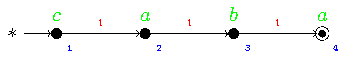
\includegraphics[width=.4\textwidth]{images/taustar.pdf}
	\caption{Graphical representation of the transition graph encoding trace $\const{caba}$.}\label{fig:taustar}

\end{figure}
%
%\begin{example}\label{ex:tracembed}
%	{Let us suppose that we want to align a trace $\tau^*$ to one of the traces from a transition graph: in order to carry out an approximate alignment, we need to transform it to a transition graph first.} A trace $\tau^*=\textup{caba}$ can be graphically represented in Figure \ref{fig:taustar}. The associated TG $T=(\mathtt{\color{blue}1},\mathtt{\color{blue}4},L,R,1)$ has matrices $L$ and $R$  defined as follows:
%	$$L:=\kbordermatrix{
%		& \texttt{\color{blue}1}&\texttt{\color{blue}2}&\texttt{\color{blue}3}&\texttt{\color{blue}4}\\
%		\color{green}a            & 0&\textbf{1}&0&\textbf{1}\\
%		\color{green}b            & 0&0&\textbf{1}&0\\
%		\color{green}c            & \textbf{1}&0&0&0\\
%	}\qquad R:=\kbordermatrix{
%		& \texttt{\color{blue}1}&\texttt{\color{blue}2}&\texttt{\color{blue}3}&\texttt{\color{blue}4}\\
%		\texttt{\color{blue}1}  & 0&\color{red}1&0&0\\
%		\texttt{\color{blue}2}  & 0&0&\color{red}1&0\\
%		\texttt{\color{blue}3}  & 0&0&0&\color{red}1\\
%		\texttt{\color{blue}4}  & 0& 0& 0& 0\\
%	}$$
%We can similarly represent all the traces from the USPN.
%\end{example}

%\begin{example}
%The subtrace \textit{\textbf{\uline{hi}}} is represented in \textit{\textbf{\uline{hi}}deous},   \textit{\uline{\textbf{h}}e\uline{{i}}d\textbf{i}}, and \textit{\uline{{\textbf{h}i}}nd\textbf{i}}, but with different frequencies and subtrace distances. We have $\embed_{\mathcal{T}}(\textit{hideous})_{{\color{green}hi}}=\lambda$,  $\embed_{\mathcal{T}}(\textit{heidi})_{{\color{green}hi}}=\lambda^2+\lambda^4$, and $\embed_{\mathcal{T}}(\textit{hindi})_{{\color{green}hi}}=\lambda+\lambda^4$.
%\end{example}



\begin{table}[t!]
\vspace{+0.7cm}
\caption{Embedding of traces $\const{caba}$, $\const{caa}$ and $\const{cb}$.}\label{tb:embedding}
\vspace{-0.4cm}
\begin{center}
\scalebox{0.6}{
	\begin{tabularx}{\textwidth}{
>{\hsize=.1\hsize}X
>{\hsize=.2\hsize}X
>{\hsize=.1\hsize}X
>{\hsize=.1\hsize}X
>{\hsize=.1\hsize}X
>{\hsize=.1\hsize}X
>{\hsize=.1\hsize}X
>{\hsize=.25\hsize}X
>{\hsize=.2\hsize}X
>{\hsize=.1\hsize}X
}
		\toprule
		& $\const{aa}$    & $\const{ab}$   & $\const{ac}$    & $\const{ba}$   & $\const{bb}$   & $\const{bc}$ & $\const{ca}$ & $\const{cb}$ & $\const{cc}$   \\
		\midrule
		$\const{caba}$ & $\lambda^2$ & $\lambda$ & $0$ & $\lambda$  & $0$  & $0$ & $\lambda+\lambda^3$ & $\lambda^2$ & $0$\\
		%$\const{caaa}$ & $2\lambda+\lambda^2$& $0$ & $0$ & $0$ & $0$ & $0$ & $\lambda+\lambda^2+\lambda^3$ & $0$ & $0$ \\
		$\const{caa}$  & $\lambda$ & $0$ & $0$ & $0$ & $0$ & $0$ & $\lambda+\lambda^2$ & $0$&  $0$\\
		$\const{cb}$   & $0$ & $0$ & $0$ & $0$ & $0$ & $0$ & $0$ & $\lambda$& $0$ \\
		\bottomrule
	\end{tabularx}
}
\vspace{-0.3cm}
\end{center}
\end{table}
\begin{example}\label{ex:wheredotiszero} %\small
Consider tasks $\tasks=\Set{a,b,c}$. The possible 2-grams over $\tasks$ are $\tasks^2=\Set{\const{aa},\const{ab},\const{ac},\const{ba},\const{bb},\const{bc},\const{ca},\const{cb},\const{cc}}$. Table~\ref{tb:embedding} shows the embeddings of some traces. Being a 2-gram, trace $\const{cb}$ has only one nonzero component, namely that corresponding to itself, with $\trembed_{\const{cb}}(\const{cb})=\lambda$. Trace $\const{caa}$ has the 2-gram $\const{ca}$ occurring with length $1$ ($\const{\underline{ca}a}$) and $2$ ($\const{\underline{c}a\underline{a}}$), and the 2-gram $\const{aa}$ with occurring length $1$ ($\const{c\underline{aa}}$). Hence: $\trembed_{\const{ca}}(\const{caa})=\lambda+\lambda^2$ and  $\trembed_{\const{aa}}(\const{caa})=\lambda$.  Similar considerations can be carried out for the other traces in the table.
We now want to compute the similarity between the first trace $\const{caba}$ and the other two traces. To do so, we sum, column by column (that is, 2-gram by 2-gram) the product of the embeddings for each pair of traces. We then get $k_{\trembed}(\const{caba},\const{caa})=\lambda^3+(\lambda+\lambda^3)(\lambda+\lambda^2)$ and $k_{\trembed}(\const{caba},\const{cb})=\lambda^3
$,
%{\footnotesize
%\[
%k_{\trembed}(\const{caba},\const{caaa})=\lambda(\lambda+\lambda^2+\lambda^3)
%~~
%k_{\trembed}(\const{caba},\const{caa})=\lambda(\lambda+\lambda^2)
%~~
%k_{\trembed}(\const{caba},\const{cb})=\lambda(\lambda+\lambda^3)
%\]}
which induces ranking $
k_{\trembed}(\const{caba},\const{caa})>
k_{\trembed}(\const{caba},\const{cb})
$.
\end{example}

\endinput
\subsection{Graph Embedding}\label{ssec:ge}
Graph kernels allow mapping graph data structures to feature spaces (usually an Euclidean space in $\mathbb{R}^n$ for $n\in \mathbb{N}_{>0}$) \cite{Samatova} so to express graph similarity functions that can then be adopted for both classification \cite{TsudaS10} and clustering algorithms. One of the first approaches used in literature involved the definition of topological description vectors \cite{Sidere} for each graph in a graph database, for then defining the graph similarity function as an inner product of their associated vectors. One inconvenience of such a technique is that it is required to perform NP-complete subgraph isomorphisms among a collection of graphs. It has been already proved that the definition of a graph kernel function fully recognizing the structure the graph always boils down to solving such NP-Complete problem \cite{GartnerFW03}, as exact embeddings generable in polynomial can be inferred just for loop-free Direct Acyclic Graphs \cite{BergamiBM20}.


Consequently, most recent literature focused on extracting relevant features of such graphs, that are then used to define a graph similarity function. The most common approach adopted in the kernel to extract such features is called \textit{propositionalization}: we might extract all the possible features (e.g., subsequences), and then define a kernel function based on the occurrence and similarity of these features \cite{Gartner03}.